\begin{savequote}[75mm] 
Nulla facilisi. In vel sem. Morbi id urna in diam dignissim feugiat. Proin molestie tortor eu velit. Aliquam erat volutpat. Nullam ultrices, diam tempus vulputate egestas, eros pede varius leo.
\qauthor{Quoteauthor Lastname} 
\end{savequote}

\chapter{Algorithm \label{chap:algorithm}}

This chapter will introduce and differentiate two types of algorithms which have been evaluated from the literature in Section \ref{sec:outlier}. Algorithms presented in Table \ref{tbl:overviewAlgorithms} are distance based algorithms, for simplicity we use Euclidean distance as in Equation \ref{eq:euclidean}, but all algorithm will also work with other metrics. For example, other metrics such as the Hamming distance, used for finding the number of different symbols in strings of equal length which is often used for comparing bit-sequences \cite{citeulike:1667687}. Another distance-function can be the Levenshtein distance which is used for comparing different text. The Euclidean distance between observation $a$ and $b$ is the length of the line segment connecting them and therefore intuitive for people to grasp \cite{Deza2009EncyclopediaofDistances}.

\begin{equation}
d({\bf a},{\bf b}) = \sqrt{\sum^{m}_{i=1} (a_{i} - b_{i})^2} \label{eq:euclidean}
\end{equation}

The distance based algorithm is related to the concept of clustering. An outlier can be seen as an observation which is not part of a cluster. Also the algorithms take the locality into account. For example, the Local Outlier Factor algorithm compares the density of the surrounding neighbours, it is important to note that the global density may vary a lot accross the feature space.

Section \ref{sec:lof} will introduce the Local Outlier Factor algorithm, which introduces the concept of local densities and has been extended and adapted by many papers. Next, the Stochastic Outlier Selection algorithm will be introduced in Section \ref{sec:sos} and why it is a good fit for Apache Spark and its implementation.

\section{Local Outlier Factor \label{sec:lof}}

Many distance-based outlier detection algorithms are based or strongly inspired by the Local Outlier Factor algorithm. The concept is depicted in Figure \ref{fig:lof} where the black dots are the observations in the feature space and the dashed circles is the corresponding distance to the $k^{\text{th}}$-point which is set to $k=3$.

\begin{figure}[ht!]
\centering
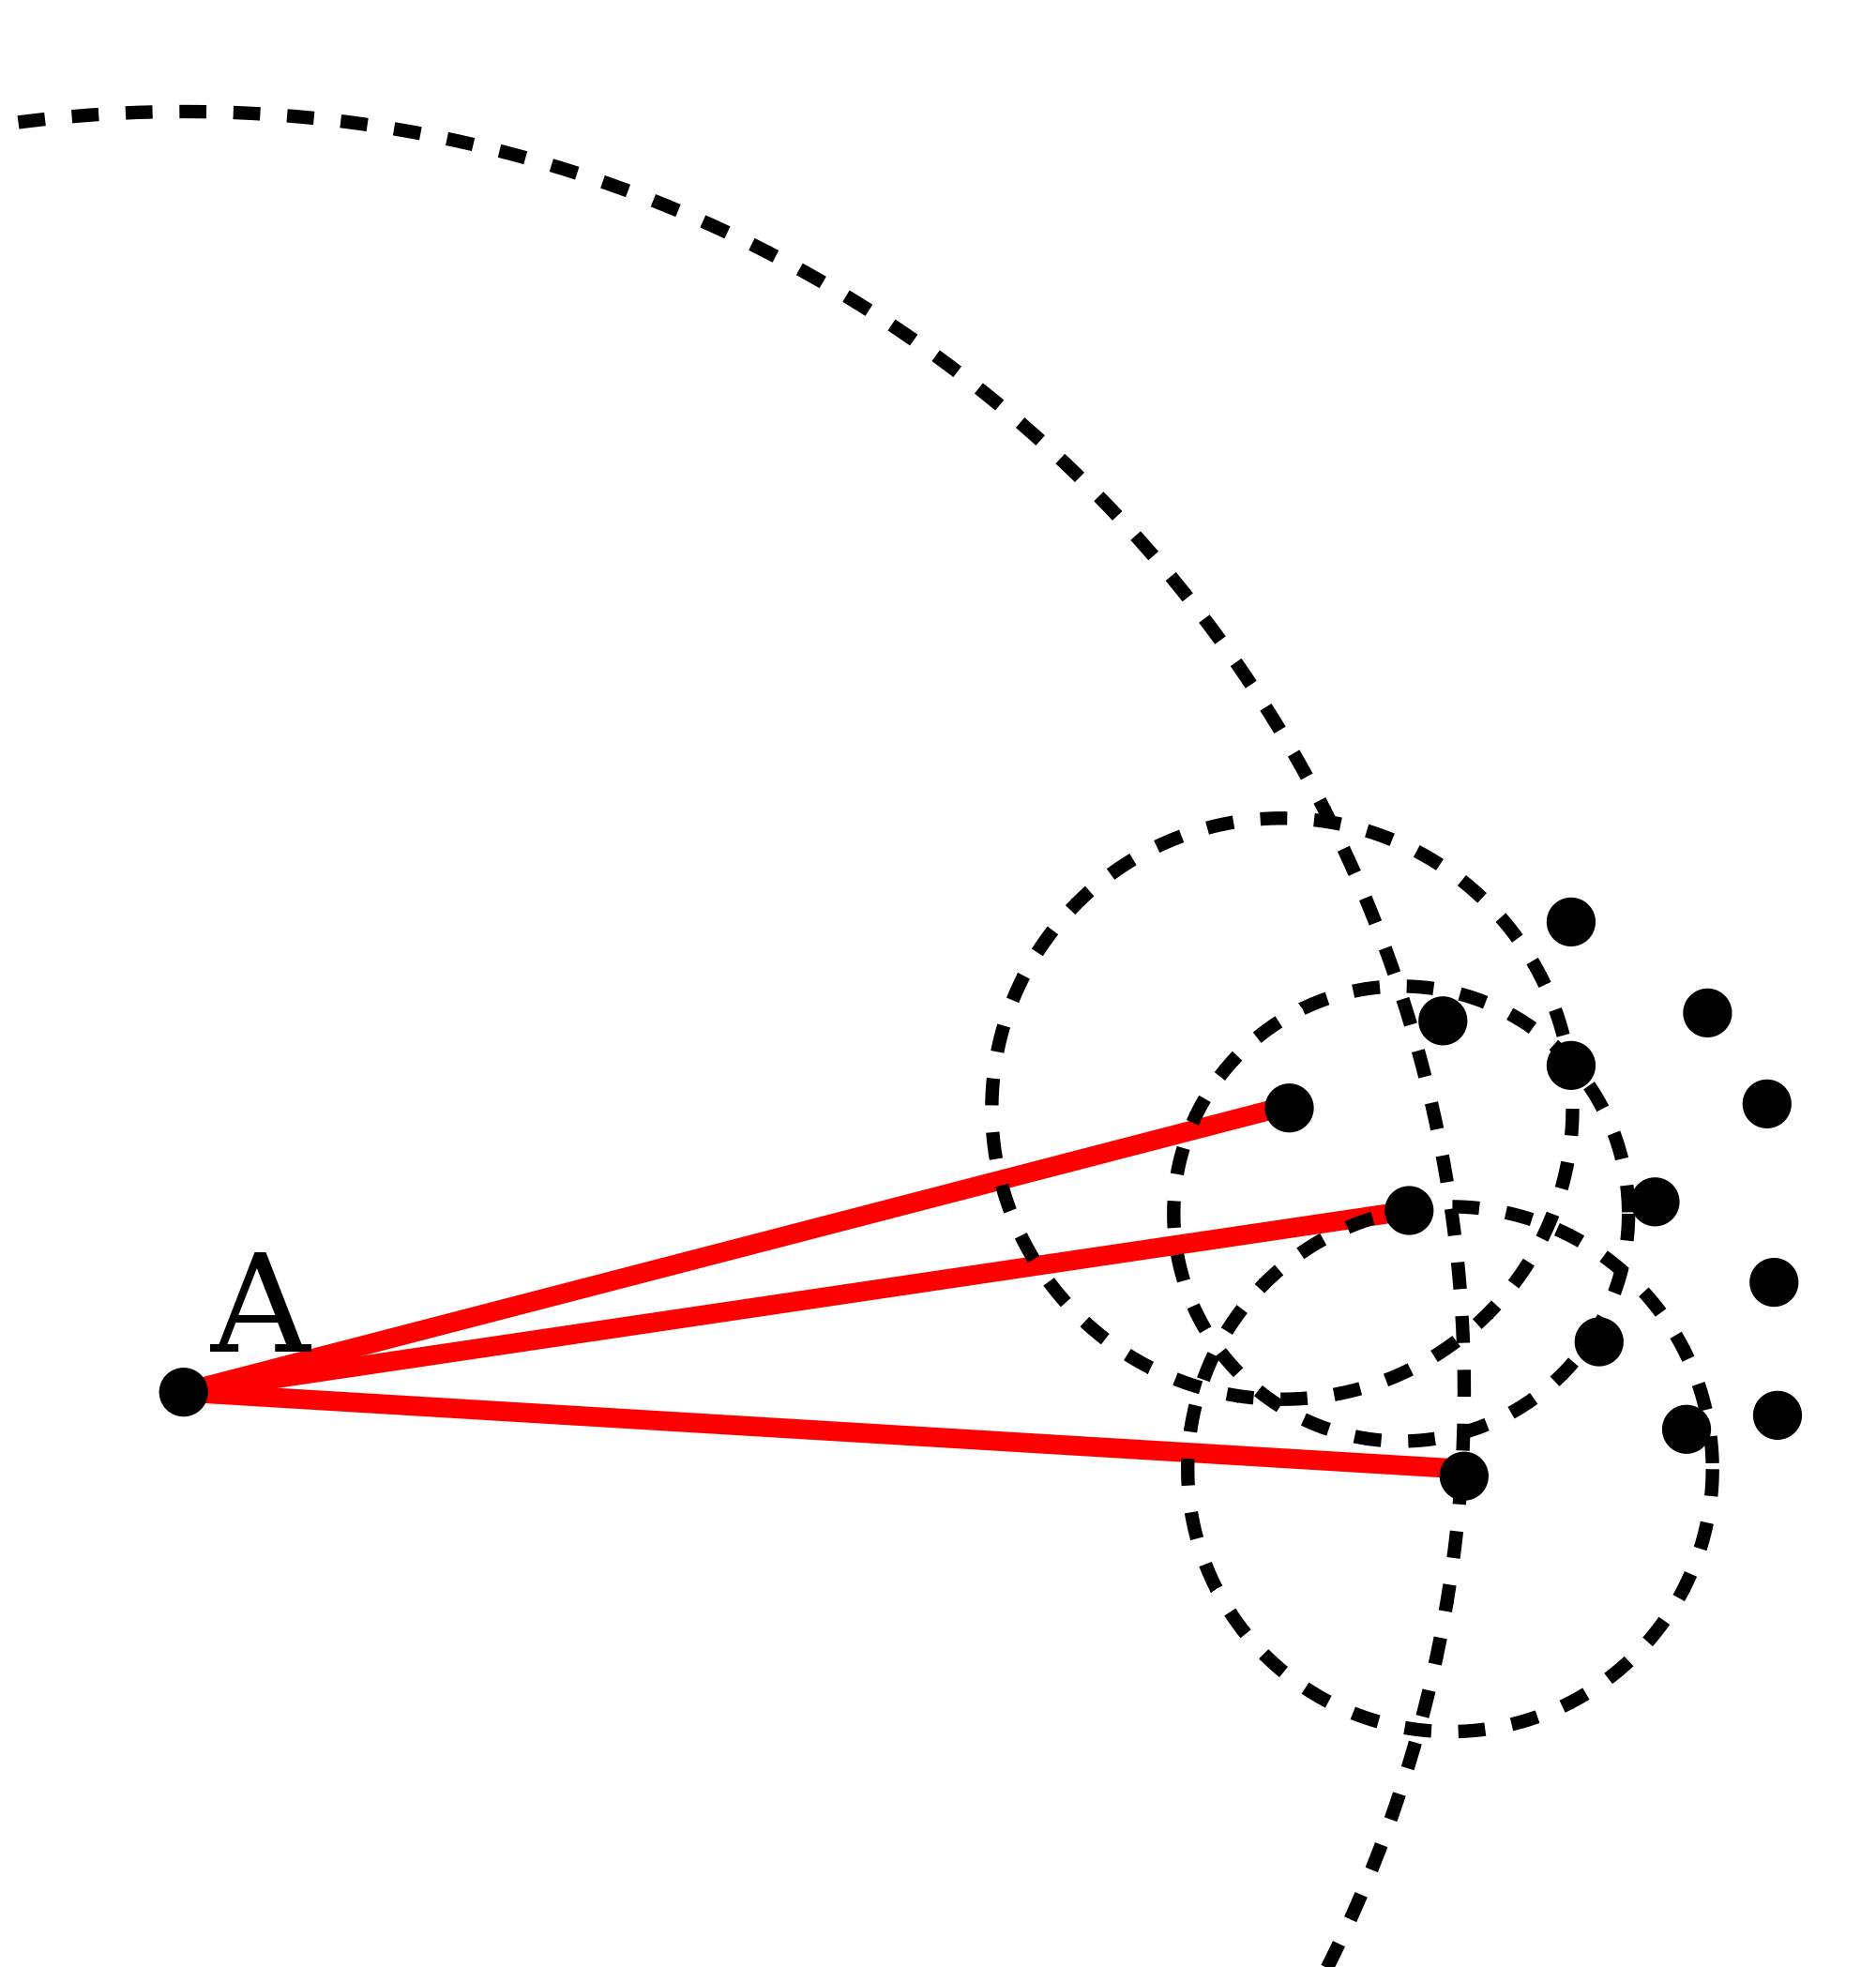
\includegraphics[width=.6\textwidth]{figures/lof.png}
\caption{Local Outlier Factor with $k=3$. \label{fig:lof}}
\end{figure}

First, the distance to the $k^{\text{th}}$-nearest observations will be computed, this is called the Local Reachability Distance (LDR) as defined in Equation \ref{eq:reachability}. Where $k\text{-distance}(A)$ is the distance to the $k^{\text{th}}$-nearest observation of the neighbouring observation $A$. 

\begin{equation}
\text{LDR}_{k}(A) = 1 / \left( \frac{\sum_{B \in N_{k}(A)} max(k\text{-distance}(B), d(A,B))}{|N_{k}(A)|} \right) \label{eq:reachability}
\end{equation}

After computing LDR for each point, which requires the $k$-nearest neighbours and the $k$-nearest neighbors of the $k$-nearest neighbors. Next, the Local Outlier Factor (LOF) can be obtained using Equation \ref{eq:lof}. Which essentially compares the local densities of the different observations.

\begin{equation}
\text{LOF}_{k}(A) = \left( \frac{\sum_{B \in N_{k}(A)} \text{LDR}(B)}{|N_{k}(A)|} \right) / \text{LDR}(A)
\label{eq:lof}
\end{equation}

The algorithm relies heavily on nearest neighbour searches which are hard to optimize on distributed computational platforms as they require to search and sort throughout all the data.

As for outlier detection algorithms, there is no free lunch \cite{Wolpert95nofree}, which implies that there is no algorithm which outperforms all other algorithms \cite{outlierselection}. Different algorithms excel under different conditions, depending on data characteristics.

\section{Stochastic Outlier Selection \label{sec:sos}}

The implementation of the Stochastic Outlier Selection algorithm has been done in Scala\footnote{Scala programming language \url{http://www.scala-lang.org/}} on top of Apache Spark.

Instead of comparing local densities as done by the Local Outlier Factor concept, the Stochastic Outlier Selection algorithm employs the concept of affinity which does comes from the field of \cite{ictdbid:2777,AISTATS09_Maaten}:

\begin{description}
  \item[Clustering] employs affinity to quantify the relationships among data observations \cite{Frey2007}. For example, the concept of affinity been used for partitioning protein interaction \cite{pmid19331680} and clustering of text \cite{10.1109/TKDE.2010.144}.
  \item[Dimensionality reduction] Stochastic Neighbor Embedding \cite{NIPS20022276} or t-distributed Stochastic Neighbor Embedding \cite{van2008visualizing,ictdbid:2777} is a nonlinear dimensionality reduction technique for embedding high-dimensional data into a space of two or three dimensions. The technique has been used among music analysis \cite{Hamel+al:2010} and bio-informatics \cite{journals/bioinformatics/WallachL09}.
\end{description}

To determine the correct working of the algorithm, unit-tests have been written to ensure correct output of each stage in the algorithm. The output of the implementation is compared to the output generated by the Python implementation written by the author\footnote{SOS \url{https://github.com/jeroenjanssens/sos/blob/master/bin/sos/}}. These unit-tests uncovered a bug in the authors' script, which has been patched by a pull request\footnote{Github pull request \url{https://github.com/jeroenjanssens/sos/pull/4/}}.

The algorithm consists of a series of transformations on the data as described in the original paper \cite{MSU:CSE:00:2}, these steps are elaborated in the following subsections and described how they are implemented.

\subsection{Distance matrix \label{subsec:distancematrix}}
The distance matrix takes the $n$ input vectors of $m$ length and transforms it to a $n \times n$ matrix by taking the pairwise distance between each vector. We employ the symmetric Euclidean distance, as defined earlier in Equation \ref{eq:euclidean}. As being symmetric sets the distance $d({\bf x}_{i},{\bf x}_{j})$ equal to $d({\bf x}_{j},{\bf x}_{i})$ and the distance to self is zero $d({\bf x}_{i},{\bf x}_{i}) = 0$. The distance matrix is denoted by ${\bf D}$, each row by ${\bf D}_{i} \in \mathbb{R}^{m}$ and each element by $D_{ij} \in \mathbb{R}$.

\begin{listing}[ht!]
\begin{minted}[frame=lines]{scala}
def computeDistanceMatrixPair(data: RDD[(Long, Array[Double])]): 
                                        RDD[(Long, Array[Double])] =
    data.cartesian(data).flatMap {
      case (a: (Long, Array[Double]), b: (Long, Array[Double])) =>
        if (a._1 != b._1)
          Some(a._1, euclDistance(a._2, b._2))
        else
          None
    }.combineByKey(
        (v1) => List(v1),
        (c1: List[Double], v1: Double) => c1 :+ v1,
        (c1: List[Double], c2: List[Double]) => c1 ++ c2
      ).map {
      case (a, b) => (a, b.toArray)
    }
\end{minted}

\caption{Computing the distance matrix of a collection of feature vectors.}
\label{list:matrixDistance}
\end{listing}

The implementation given in Listing \ref{list:matrixDistance} takes the Cartesian product of the input vectors to compute every pair distance. Next the pairs are mapped to compute Euclidean the distance between every pair of vectors, except to itself as it does not carry any information for the algorithm. Finally all the vectors are combined by the unique key of each vector returning the rows of the matrix.

\subsection{Affinity matrix \label{subsec:affinity}}
The affinity matrix will be obtained by transforming the distance matrix and is proportional to the distance between two data observations. The affinity quantifies the relationship from one data point to another data point. The affinity $\sigma_{i}$ for each point is found by performing binary search, which makes the entropy of the distribution over all neighbors equal to the logarithm of the perplexity parameter $h$.

\begin{equation}
a_{ij} = \begin{cases} \exp(-d_{ij}^{2} / 2 \sigma_{i}^{2}) & \text{if } i \neq j\\ 0 & \text{if } i = j \end{cases}
\label{eq:affinity}
\end{equation}

The perplexity parameter is the only configurable parameter for the algorithm denoted by $h$ as in Equation \ref{eq:perplexity}. The influence of the $h$ parameter is comparable to the $k$ parameter in $k$-nearest neighbours (KNN). It alters the behaviour of the algorithm analogously, the higher the value $h$, the more it will depend on the surrounding neighbours. One important difference is that $h \in \mathbb{R}$ and $k \in \mathbb{N}$. The perplexity value has a deep foundation in information theory, but in practice should it be tuned by the domain expert to provide a good level of outlierness \cite{MSU:CSE:00:2}.

\begin{listing}[ht!]
\begin{minted}[frame=lines]{scala}
def computeAffinityMatrix(dMatrix: RDD[(Long, Array[Double])], 
                          perplexity: Double = DEFAULT_PERPLEXITY): 
                                  RDD[(Long, DenseVector[Double])] = 
  dMatrix.map(r => (r._1, binarySearch(new DenseVector(r._2), Math.log(perplexity))))
\end{minted}
               
\caption{Transforming the distance matrix to the affinity matrix.}
\label{list:matrixAffinity}
\end{listing}

Listing \ref{list:matrixAffinity} invokes the binary search which approximates the affinity based on each row within the matrix. The maximum number of iterations can be set to interrupt the execution as some point, also a tolerance can be set to accept a small error in exchange for reduced computational time.

\begin{equation}
h = \{x \in \mathbb{R} | 1 \leq x \leq n-1\}
\label{eq:perplexity}
\end{equation}



The affinity matrix is obtained by applying Equation \ref{eq:affinity} on every element of the distance matrix. Perplexity is employed to set adaptively the variances which is computed using a search so that every point has effectively $h$ neighbours \cite{NIPS20022276}. Assuming that each point has an unique place in space, then for each point the standard deviation value $\sigma^{2}$ has to be approximated. The values of the variances that correspond to the desired perplexity are found using a binary search. The binary search iteratively bisects the interval and then selects the correct upper of lower half until the desired variances for each data point are found.

\begin{listing}[ht!]
\begin{minted}[frame=lines]{scala}
def binarySearch(affinity: DenseVector[Double],
                 logPerplexity: Double,
                 iteration: Int = 0,
                 beta: Double = 1.0,
                 betaMin: Double = Double.NegativeInfinity,
                 betaMax: Double = Double.PositiveInfinity,
                 maxIterations: Int = DEFAULT_ITERATIONS,
                 tolerance: Double = DEFAULT_TOLERANCE): DenseVector[Double] = {

  val newAffinity = affinity.map(d => Math.exp(-d * beta))
  val sumA = sum(newAffinity)
  val hCurr = Math.log(sumA) + beta * sum(affinity :* newAffinity) / sumA
  val hDiff = hCurr - logPerplexity

  if (iteration < maxIterations && Math.abs(hDiff) > tolerance) {
    val search = if (hDiff > 0)
      (if (betaMax == Double.PositiveInfinity || betaMax == Double.NegativeInfinity)
        beta * 2.0
      else
        (beta + betaMax) / 2.0, beta, betaMax)
    else
      (if (betaMin == Double.PositiveInfinity || betaMin == Double.NegativeInfinity)
        beta / 2.0
      else
        (beta + betaMin) / 2.0, betaMin, beta)

    binarySearch(   affinity,
                    logPerplexity, 
                    iteration + 1, 
                    search._1, 
                    search._2, 
                    search._3, 
                    maxIterations, 
                    tolerance)
  }
  else
    newAffinity
}
\end{minted}
\caption{Performing a binary search to approximate the affinity for each point.}
\label{list:approximateAffinity}
\end{listing}

Listing \ref{list:approximateAffinity} shows the recursive function to find or approximate the perplexity of each row $x_{i}$ in the distance matrix. The recursive function eliminates mutable variables which are impossible to avoid when using using loops. The use of immutable variables comes from the functional programming aspect of Scala and makes the code less error prone.

Another setting of the search is to set a predefined tolerance at which the search will stop when the remaining error is within a certain range. This setting will introduce some error and therefore decrease precision, but can help to reduce the computational time. The remaining error gets reduced by half each iteration, therefore the last few iterations have little influence on the final result. When execution time is an important factor, a small tolerance can be introduced.

\subsection{Binding probability matrix \label{subsec:bindingprob}}

The binding probability matrix defines the probability that observation $x_{i}$ to $x_{j}$. The mathematical foundation based on graph theory computes the Stochastic Neighbour Graph and the subsequently generative process is out of scope and can be found in its original paper \cite{MSU:CSE:00:2}.

\begin{equation}
b_{ij} = \frac{a_{ij}}{\sum_{k=1}^{n}a_{ik}}
\label{eq:binding}
\end{equation}

The binding probability matrix can be applied by normalizing the affinity matrix such that $\sum_{k=1}^{n}$ sums up to $1$. Equation \ref{eq:binding} will transform the affinity matrix to the probability outlier matrix.

\begin{listing}[ht!]
\begin{minted}[frame=lines]{scala}
def computeBindingProbabilities(rows: RDD[(Long, DenseVector[Double])]): 
                                            RDD[(Long, Array[Double])] = 
  rows.map(r => (r._1, r._2 :/ sum(r._2)).toArray)
\end{minted}

\caption{Transforming the affinity matrix into the binding probability matrix.}
\label{list:matrixProbability}
\end{listing}

Listing \ref{list:matrixProbability} shows the implementation that divides each element by the sum of the vector.

\subsection{Computing outlier probabilities \label{subsec:outlierprobabilities}}

The last step is computing the outlier probability of vector ${\bf x}_{i}$, which is given by the product of the column binding probability matrix as in Equation \ref{eq:final}.

\begin{equation}
f{_\text{SOS}}({\bf x}_{i}) \equiv \prod^{n}_{\substack{i=1\\j \neq i}}(1-b_{ji}) \label{eq:final}
\end{equation}

The implementation is given in Listing \ref{list:matrixOutput}. The implementation uses a \texttt{flatmap} to add indices to the elements of the vector. The inline if condition will offset the indices with one to skip the diagonal of the matrix. Important to note is the \texttt{zipWithIndex} operation is applied to the local collection and not on the RDD which would trigger an expensive Spark job.

\begin{listing}[ht!]
\begin{minted}[frame=lines]{scala}
def computeOutlierProbability(rows: RDD[(Long, Array[Double])]):
                                                    RDD[(Long, Double)] =
  rows.flatMap(r => r._2.zipWithIndex.map(p =>
    (p._2 + (if (p._2 >= r._1) 1L else 0L), p._1))).foldByKey(1.0)((a, b) => a * (1.0 - b))
\end{minted}

\caption{Computing the outlierness from the binding probability matrix.}
\label{list:matrixOutput}
\end{listing}

Finally the \texttt{foldByKey} will group all the keys and perform a fold which will compute the product of each column. This last action will invoke a data-shuffle as the rows are distributed across the different worker nodes.